\documentclass{beamer}
\usepackage{tcolorbox}
\usepackage{hyperref}
\usepackage{../../../shared/notation/notation}

%\beamerdefaultoverlayspecification{<+->}
% \newcommand{\data}{\mathcal{D}}
% \newcommand\Item[1][]{%
% 	\ifx\relax#1\relax  \item \else \item[#1] \fi
% 	\abovedisplayskip=0pt\abovedisplayshortskip=0pt~\vspace*{-\baselineskip}}

\graphicspath{ {imgs/} }

\usetheme{metropolis}           % Use metropolis theme


\title{KKT Conditions}
\date{\today}
\author{Nipun Batra}
\institute{IIT Gandhinagar}
\begin{document}
	\maketitle

	\begin{frame}{KKT Conditions}
	Used for constrained optimization of the form\\
	\vspace{1cm}
	Minimize $f(x)$, where $x \in \mathbb{R}^k$\\
	such that\\
	\begin{center}
	$h_i(x) = 0$,  $\forall i = 1, \dots, m$ (m equalities)\\
	$g_j(x) \leq 0$,  $\forall j = 1, \dots, n$ (n inequalities)\\
	\end{center}
	\end{frame}

	\begin{frame}{Step 1}
	\begin{itemize}
	\only<1->{
	\item Create a new function for minimization, \\
	\vspace{0.5cm}
	$L(x, \lambda_1, \dots, \lambda_m, \mu_1, \dots, \mu_n ) = f(x) + \sum\limits_{i=1}^{m}\lambda_ih_i(x) + \sum\limits_{j=1}^{n}\mu_jg_j(x)$\\
	\vspace{0.5cm}
	where,\\ $\lambda_1-\lambda_m$ are multipliers for the $m$ equalities \\
	$\mu_1-\mu_n$ are multiplices for the $n$ inequalities \\
	}
	\end{itemize}
	\end{frame}

	\begin{frame}{Step 2}
	\begin{itemize}
	\item Minimize $L(x, \lambda, \mu)$ w.rt. $x \implies \nabla_xL(x, \lambda, \mu) = 0 $\\
	Gives $k$ equations
	\end{itemize}
	\end{frame}

	\begin{frame}{Step 3}
	\begin{itemize}
	\item Minimize $L(x, \lambda, \mu)$ w.rt. $\lambda \implies \nabla_\lambda L(x, \lambda, \mu) = 0 $\\
	Gives $m$ equations
	\end{itemize}
	\end{frame}

	\begin{frame}{Step 4}
	\begin{columns}
		  \begin{column}{0.5\textwidth}
			
\includegraphics[width = \textwidth]{img1}
			\centering
			$g_i(x^*) \leq 0$\\
			$\mu_i = 0$
		  \end{column}
		  \begin{column}{0.5\textwidth}
			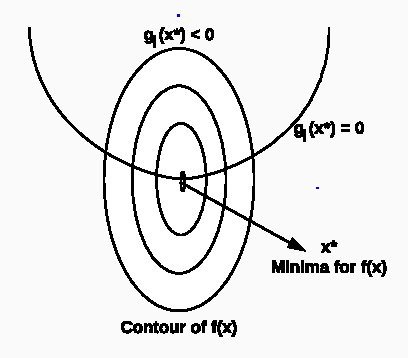
\includegraphics[width = \textwidth]{img2}
			\centering
			$g_i(x^*) = 0$
		  \end{column}
	\end{columns}
	\vspace{1cm}
	\centering
	In both cases, $\mu_ig_i(x^*) = 0$
	\end{frame}

	\begin{frame}{Constraint on $\mu_i$'s}
	\centering
	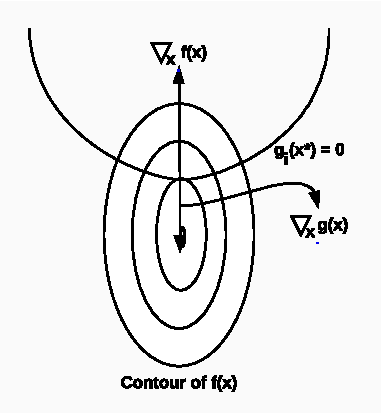
\includegraphics[width = 0.5\textwidth]{img3}
	$min_xL(x, \lambda, \mu)  \implies \nabla_xf(x) + \nabla_x\mu_ig_i(x) = 0$\\
	\vspace{0.5cm}
	$\mu_i = \dfrac{\nabla_xf(x)}{\nabla_x\mu_ig_i(x)} = +ve$
	\end{frame}

	\begin{frame}{KKT Conditions}
	\only<1->{
	\textbf{Stationarity (For minimization)}\\
	$\nabla_xf(x) + \sum\limits_{i=1}^m\nabla_x\lambda_ih_i(x)  + \sum\limits_{i=1}^n\nabla_x\mu_ig_i(x) = 0$ \\
	\vspace{0.5cm}
	}
	\only<2->{
	\textbf{Equality Constraints}\\
	$\nabla_\lambda f(x) + \sum\limits_{i=1}^m\nabla_\lambda\lambda_ih_i(x)  + \sum\limits_{i=1}^n\nabla_\lambda\mu_ig_i(x) = 0$ \\
	$\sum\limits_{i=1}^m\nabla_\lambda\lambda_ih_i(x)  = 0$\\
	}
	\only<3->{
	\vspace{0.5cm}
	\textbf{Inequality Constraints (Complementary Slackness)}\\
	$\mu_ig_i(x) = 0 \forall i = 1,\dots, n$\\
	$\mu_i \geq 0$
	}	
	\end{frame}

	\begin{frame}{Example}
	Minimize $x^2 + y^2$ such that,\\
	\centering
	$x^2 + y^2 \leq 5$\\
	$x + 2y = 4$\\
	$x,y \geq 0$
	\end{frame}

	\begin{frame}{Example}
	\only<1->{
	$f(x,y) = x^2 + y^2$\\
	}
	\only<2->{
	$h(x,y) = x + 2y - 4$\\
	}
	\only<3->{
	$g_1(x,y) = x^2 + y^2 - 5$\\
	}
	\only<4->{
	$g_2(x,y) = -x$\\
	}
	\only<5->{
	$g_3(x,y) = -y$\\
	}
	\only<6->{
	\vspace{1cm}
	$L(x,y, \lambda, \mu_1, \mu_2, \mu_3) = x^2 + y^2 + \lambda(x + 2y - 4) + \mu_1(x^2 + y^2 - 5) + \mu_2(-x) + \mu_3(-y)$\\
	}
	\end{frame}

	\begin{frame}{Example}
	\only<1->{
	\textbf{Stationarity}\\
	$\nabla_xL(x,y, \lambda, \mu_1, \mu_2, \mu_3)  = 0$\\
	$\implies 2x + \lambda + 2\mu_1x - \mu_2 = 0 \dots\dots\dots\dots\dots\dots (1)$\\
	\vspace{0.5cm}
	$\nabla_yL(x,y, \lambda, \mu_1, \mu_2, \mu_3)  = 0$\\
	$\implies 2y + 2\lambda + 2\mu_1y - \mu_3 = 0 \dots\dots\dots\dots\dots\dots (2)$\\
	}
	\only<2->{
	\vspace{0.5cm}
	\textbf{Equality Constraint}\\
	$x + 2y = 4 \dots\dots\dots\dots\dots\dots\dots\dots\dots\dots\dots\dots (3)$\\	
	}
	\only<3->{
	\vspace{0.5cm}
	\textbf{Slackness}\\
	$\mu_1(x^2 + y^2 - 5) = 0 \dots\dots\dots\dots\dots\dots\dots\dots\dots (4)$\\
	$\mu_2x = 0 \dots\dots\dots\dots\dots\dots\dots\dots\dots\dots\dots\dots\dots (5)$\\
	$\mu_3y = 0 \dots\dots\dots\dots\dots\dots\dots\dots\dots\dots\dots\dots\dots (6)$
	}
	\end{frame}

	\begin{frame}{Example}
	\only<1->{
	From (6), $\mu_3 = 0$ or $y = 0$\\
	But if, $y = 0$, then $x = 4$ according to (3) . This violates (1).\\
	Hence, $y \neq 0$ and $\mu_3 = 0$\\
	\vspace{0.5cm}
	}
	\only<2->{
	From (5), $\mu_1 = 0$ or $x = 0$\\
	If $x = 0$, $y = 2$, which implies $x^2 + y^2 = 4 (\leq 5)$ \\
	Since (x,y) = (0,2) gives smaller $x^2 + y^2$ terms than 5, \\
	Using (4), $\mu_1 = 0$\\
	}
	\only<3->
	{
	\vspace{0.5cm}
	On further solving we get,\\
	$x = 0.8$\\
	$y = 1.6$\\
	}
	\end{frame}

\end{document}